\section{Эволюция вселенной: основные наблюдательные свидетельства}

Hubble Ultra-Deep Field -— изображение небольшого региона космоса, составленное из данных, полученных космическим телескопом «Хаббл».


\begin{wrapfigure}[20]{r}{0.6\linewidth}
  \centering
    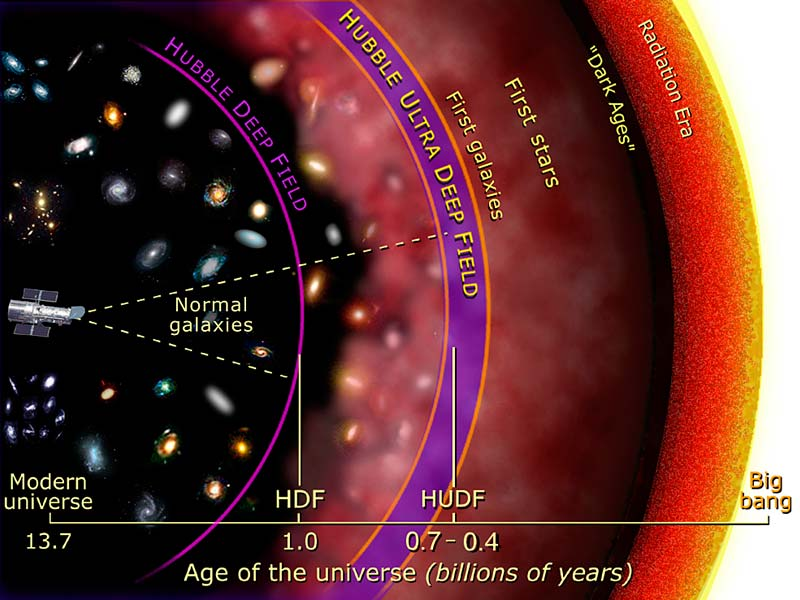
\includegraphics[width=\linewidth]{Pictures/19_hubble.jpg}
  \caption{Диаграмма, отражающая дальность видимости Хаббла}
  \label{fig:19_hubble}
 \end{wrapfigure}
Для обзора была выбрана область неба с низкой плотностью ярких звёзд в ближней зоне, что позволило лучше разглядеть более далёкие и тусклые объекты. Изображение охватывает участок неба диаметром чуть больше 3 угловых минут (1/13 000 000 от всей площади неба), и содержит примерно 10000 галактик.

Типичное расстояние до галактики на глубоком поле Хаббла составляет примено половину возаста Вселенной, следовательно, мы видим далекие галактики молодыми, еще не сформировавшимися.

\subsection{Формирование галактик}

Формы таких дальних галактик довольно причудливые по сравнению с близкими галактиками, так как они взаимодействуют между собой, что стимулирует звездообразования (формируются звёзды из верхнего левого угла диаграммы Герцшпрунга-Рассела \ref{fig:9_diag}).

Это является признаком эволюции вселенной, так как мы можем \textbf{отслеживать темп звездообразования}.
\begin{wrapfigure}[13]{r}{0.3\linewidth}
  \centering
    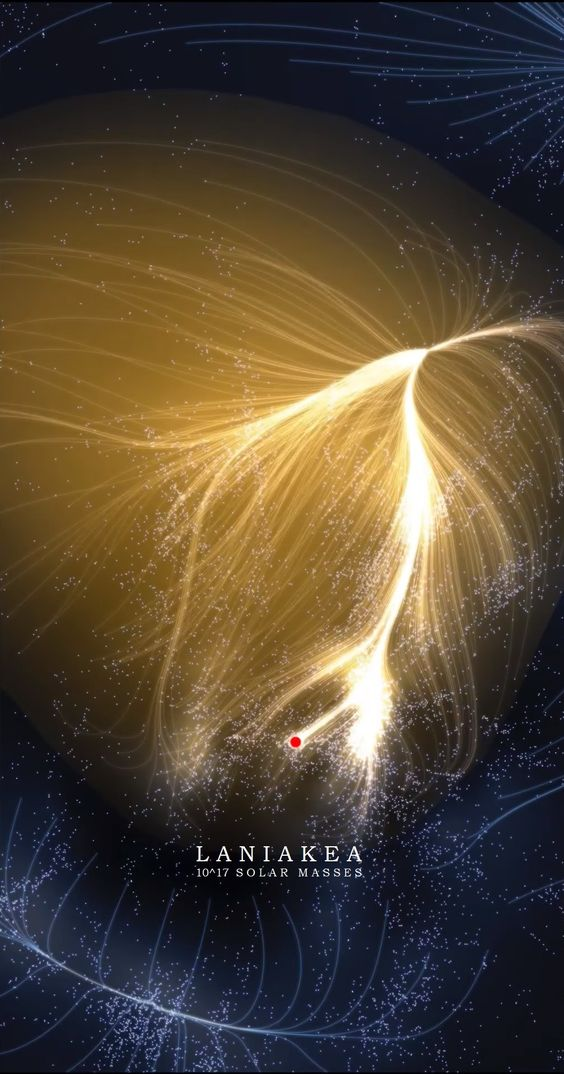
\includegraphics[width=0.7\linewidth]{Pictures/19_lan.jpg}
  \caption{Ланиакея}
  \label{fig:19_lan}
 \end{wrapfigure}
\subsection{Формирование скоплений}

Другим объектом для рассмотрения можно взять скопления галактик на разных расстояниях от нас. Сравнивая разные скопления на разных этапах их формирования, в том числе и эпоху, когда скопления галактик ещё не возникли (1-2 млрд. лет после Большого Взрыва).

\subsection{Ланиакеа}

На расстоянии $\sim 100$ млн. световых лет (что довольно мало) можно довольно точно изучить распределение скоростей галактик (проекций скоростей на луч зрения). Ланиакея (или Ланиакеа) -- это формирующееся сверхскопление галактик, в которую войдут десятки тысяч крупных галактик. Линии -- это треки, а координаты отражают космологические (связанные с расширением вселенной) скорости, которые можно оценить по закону Хаббла. Диаметр Ланиакеи примерно равен 520 миллионам световых лет.

\subsection{Дипольный отталкиватель}
Центр эффективного отталкивания в крупномасштабном течении галактик, находящихся вблизи Млечного Пути, это большие масштабы по сравнению с Ланиакеей: структура, простирающаяся от сверхскопления Шепли до Дипольного отталкивателя, имеет длину почти 1,7 миллиардов световых лет и в 2017 году стала крупнейшим картографированным объектом в наблюдаемой Вселенной. 
\begin{figure}[h]
  \centering
    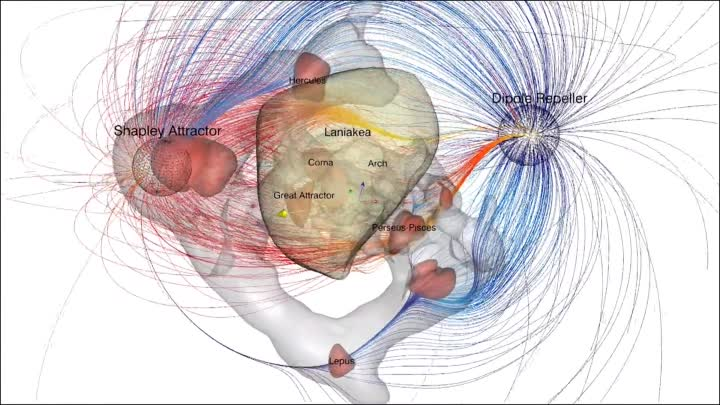
\includegraphics[width=0.7\linewidth]{Pictures/19_dip.jpg}
  \caption{Дипольный отталкиватель и сверхскопление Шепли}
  \label{fig:19_dip}
 \end{figure}
 Этот объект говорит о том, что вселенная эволюционирует, так как мы говорим об изменении морфологии галактик и является важным источником информации.
 
 \subsection{Химическая эволюция}
 
 Есть множевство процессов, приводящих к тому, что легкие элементы превращаются в тяжелые. Изучение областей Вселенной (не только звёзд, но и облаков), но обогащенных тяжелыми элементами, является объектом исследований.
 
 \subsection{Реликтовое излучение}
 
 Можно исследовать эволюцию, измеряя температуру реликтового излучения в разные моменты времени с помощью \textbf{эффекта Сюняева - Зельдовича}.
 После рекомбинации вся Вселенная всегда была заполнена реликтовым излучением, которое имеет спектр, а значит, ему в соответствие можно поставить температуру.
 
 Рассмотрим скопление галактик, где имеется горячий газ, излучающий в рентгеновском диапазоне, а значит, есть электроны с большими скоростями. Фотоны реликтового излучения, имеющие меньшую энергию, будут рассеиваться на этих электронах $\implies$ приобретать энергию. Измеряя реликтовое излучение, мы можем измерить красное смещение (фотоны перебегут на более короткие длины волн). 
 
 По эффекту рассеяния, зная температуру газа в скоплении, мы можем измерить температуру реликтового излучения в разные эпохи.
 
 \begin{figure}
  \centering
    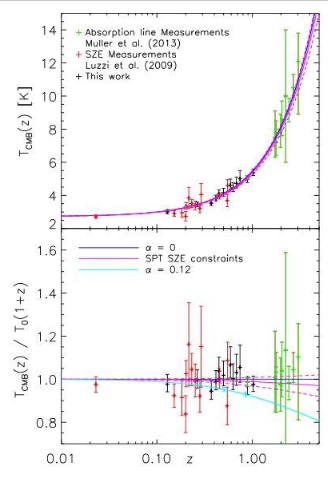
\includegraphics[width=0.5\textwidth]{Pictures/19_imdone.png}
  \caption{Эволюция температуры реликтового излучения}
  \label{fig:19_done}
 \end{figure}